\documentclass[11pt,a4paper]{article}

\usepackage[utf8]{inputenc}
\usepackage[T1]{fontenc}
\usepackage[english]{babel}
\usepackage{lmodern}
\usepackage{geometry}
\usepackage{graphicx}
\usepackage{booktabs}
\usepackage{float}
\usepackage{amsmath}
\usepackage{microtype}
\usepackage[authoryear]{natbib}
\usepackage[colorlinks=true,linkcolor=black,citecolor=black,urlcolor=blue]{hyperref}

\geometry{margin=2.5cm}
\graphicspath{{../../figures/}}
\setlength{\parskip}{0.6em}
\setlength{\parindent}{0pt}

\title{LLMs Under the Microscope:\\Uncertainty, Statistical Power, and the Illusion of Exact Ranking}
\author{Diego Henrique Xavier}
\date{2026}

\begin{document}

\maketitle

\begin{abstract}
Public leaderboards of language models usually treat differences of a few tenths of a percentage point as if they were precise facts. This project re-examines that assumption by treating benchmark scores as finite-sample estimates rather than exact measurements. Using 4,496 models from Open LLM Leaderboard v2 and about 33 thousand battles from the LMSYS Chatbot Arena, the analysis applies Wilson confidence intervals, non-parametric bootstrap, pairwise tests with Benjamini--Hochberg correction, statistical power analysis, Bradley--Terry modeling, and Elo-style comparisons. The results show that the theoretical margin of error in GPQA exceeds \(\pm 4.6\) percentage points near \(p=0.5\), that more than 60\% of top-100 pairs in that benchmark are statistically indistinguishable, and that multiple-comparison correction sharply reduces the fraction of significant differences among top-ranked models. Metadata alone explains about \(R^2 \approx 0.70\) of leaderboard average through XGBoost, while the Arena qualitatively agrees with leaderboard ordering on the overlapping models. The main implication is practical: exact position is often a reporting artifact, and model choice is better framed in terms of statistical tiers.
\end{abstract}

\textbf{Keywords:} language models; leaderboards; binomial inference; bootstrap; Bradley--Terry; Chatbot Arena.

\section{Introduction}
Public LLM rankings are commonly read as if rank 1 is meaningfully different from rank 5 even when the gap is a fraction of a percentage point. That interpretation is weak when each benchmark score is only an estimate computed from a finite set of questions. If a benchmark contains \(n\) items, the observed score is a binomial proportion subject to sampling variability. Once uncertainty is made explicit, many of the apparent fine-grained differences become fragile.

This study asks a direct question: how much of what is published as a leaderboard survives conventional statistical scrutiny? The answer matters because leaderboards increasingly guide production choices, research narratives, and claims about model progress.

The project has four goals:
\begin{enumerate}
    \item quantify uncertainty in public benchmark scores with interval estimates;
    \item test whether adjacent top models are statistically separable after multiple-comparison correction;
    \item assess whether current benchmark sizes have enough power to support fine-grained ranking claims;
    \item compare benchmark ordering with human-preference data from the Arena.
\end{enumerate}

\section{Background}
The statistical core of the problem is simple. Benchmark accuracy can be written as \(\hat{p}=k/n\), where \(k\) is the number of correct items out of \(n\) questions. For interval estimation, this work uses Wilson score intervals \citep{wilson1927}, which are generally better behaved than the classical Wald interval, especially away from the center and at moderate sample sizes \citep{agresti1998}. For communication and top-rank visualization, non-parametric bootstrap \citep{efron1979} is also used.

Pairwise comparisons create a second problem. A top-50 list implies \(50\times49/2 = 1{,}225\) simultaneous tests. Without correction, many apparently significant differences are expected by chance. To address this, the analysis uses false-discovery-rate control with the Benjamini--Hochberg procedure \citep{benjamini1995}. Effect size is reported with Cohen's \(h\) for proportions \citep{cohen1988}.

For Arena battles, ranking is modeled with Bradley--Terry \citep{bradley1952} estimated by the MM procedure of \citet{ford1957}. Ratings are also interpreted on an Elo-like scale for readability \citep{elo1978}. The leaderboard and the Arena are complementary: the first is based on structured benchmarks, while the second is based on blinded human preference comparisons \citep{zheng2023arena,arena2026}.

\section{Data and Methods}

\subsection{Data sources}
The benchmark side of the study uses Open LLM Leaderboard v2 \citep{huggingface2024leaderboard}, after removing entries flagged by the leaderboard maintainers. The cleaned analytic base contains 4,496 models and six core benchmarks: IFEval, BBH, MATH Lvl 5, GPQA, MuSR, and MMLU-PRO. Metadata such as parameter scale, architecture family, precision, and organization were parsed from the published model identifiers.

The preference side uses approximately 33 thousand battles from the LMSYS Chatbot Arena ecosystem \citep{zheng2023arena,arena2026}. Ties were excluded from the main Bradley--Terry fit so that each retained battle represented a decisive comparison.

\subsection{Statistical pipeline}
The codebase is organized into ten sequential steps: ingestion, preprocessing, auditing, exploratory analysis, inference, machine learning, ranking, Arena modeling, and consolidated reporting. The main parameters are:
\begin{itemize}
    \item Wilson intervals at 95\% confidence;
    \item bootstrap with 2,000 resamples for leaderboard ranking plots;
    \item Benjamini--Hochberg correction at \(\alpha = 0.05\);
    \item power analysis at \(\alpha = 0.05\) and power \(= 0.80\);
    \item Bradley--Terry fit with bootstrap confidence intervals in the Arena slice.
\end{itemize}

\subsection{Derived quantities}
Three derived quantities drive the interpretation:
\begin{enumerate}
    \item the theoretical margin of error implied by each benchmark size;
    \item the share of top-ranked pairs whose differences are too small to be distinguished;
    \item the number of items that would be required to reliably separate top models when the observed gap is used as the effect size.
\end{enumerate}

\section{Results}

\subsection{Benchmark size governs uncertainty}
The first result is mechanical but decisive. Benchmark length is not a side detail; it defines the precision of the ranking. GPQA, with only 448 questions, implies a much wider error band than MMLU-PRO, which contains 12,032 items.

\begin{table}[H]
\centering
\caption{Benchmark size and theoretical Wilson margin of error at \(p=0.5\)}
\begin{tabular}{lrr}
\toprule
Benchmark & \(n\) & MOE (pp) \\
\midrule
GPQA & 448 & 4.6 \\
IFEval & 541 & 4.2 \\
MuSR & 756 & 3.6 \\
MATH Lvl 5 & 1,324 & 2.7 \\
BBH & 6,511 & 1.2 \\
MMLU-PRO & 12,032 & 0.9 \\
\bottomrule
\end{tabular}
\end{table}

\begin{figure}[H]
\centering
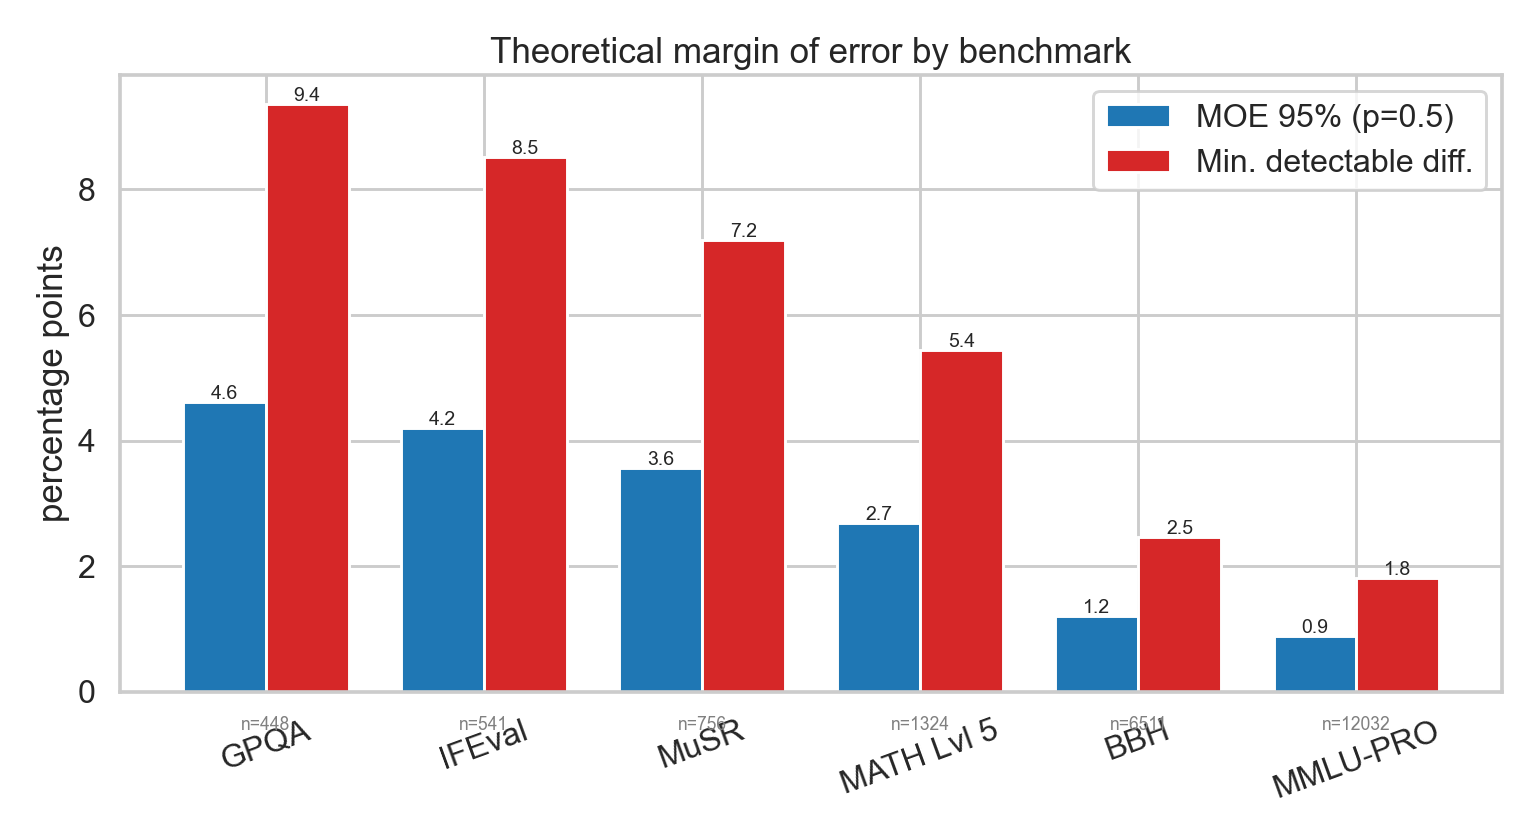
\includegraphics[width=0.8\textwidth]{04_moe_teorica.png}
\caption{Theoretical margin of error by benchmark.}
\end{figure}

This scale difference changes the meaning of rank interpretation. In GPQA, a three-point gap can easily be smaller than the uncertainty around each estimate. In MMLU-PRO, the same gap is much easier to defend.

\subsection{Most top pairs are not clearly separable}
The project estimates how many pairs in the top-100 have differences smaller than the minimum detectable effect implied by their benchmark size. GPQA and MuSR are the clearest warnings: most pairwise gaps at the top are too small to sustain deterministic ordering.

\begin{figure}[H]
\centering
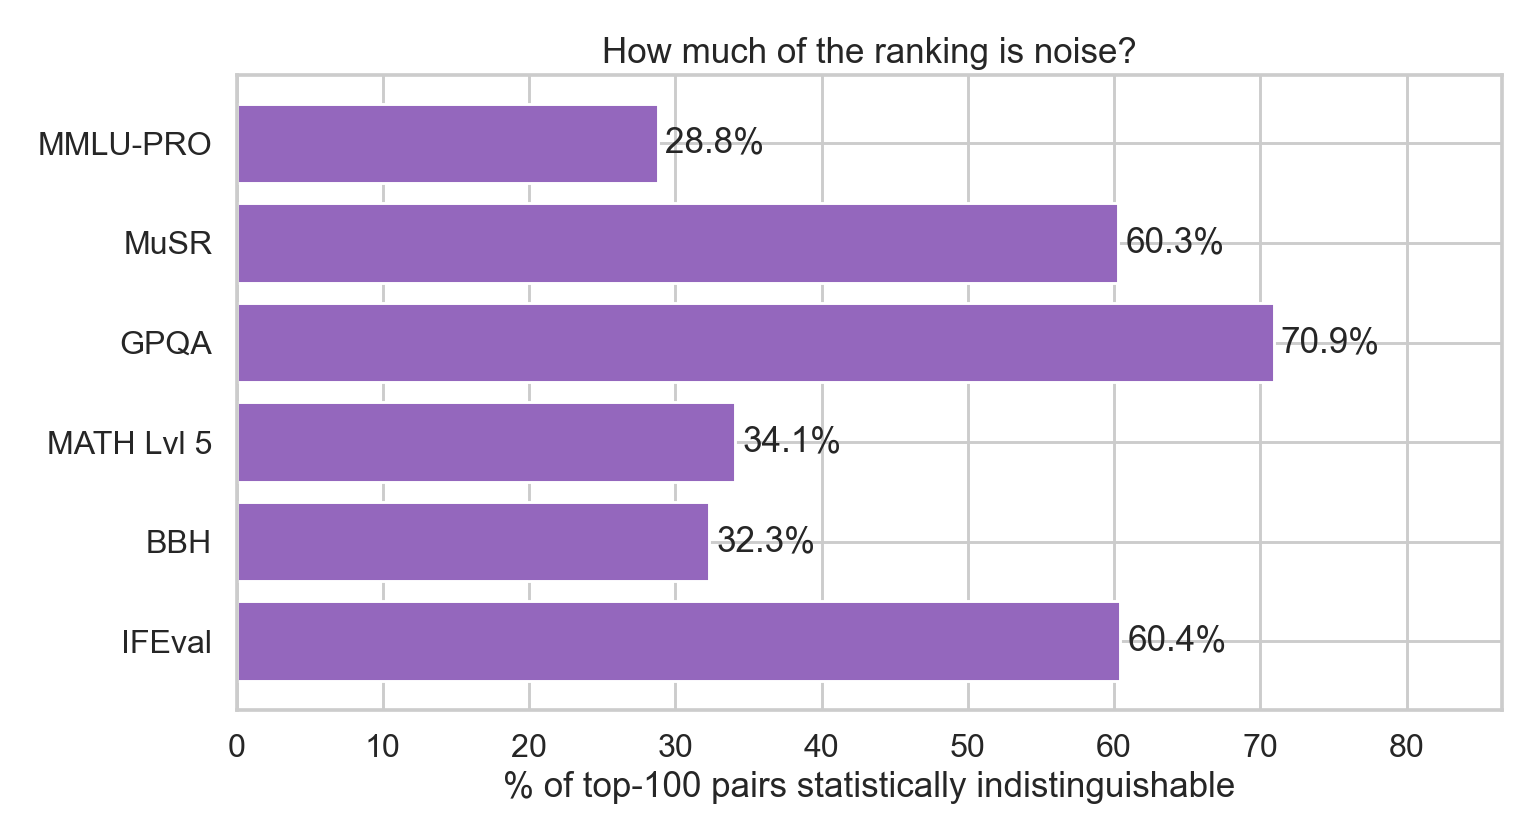
\includegraphics[width=0.8\textwidth]{04_pct_pares_indistinguiveis.png}
\caption{Share of statistically indistinguishable pairs in the top-100.}
\end{figure}

The practical reading is straightforward. A leaderboard may list one model above another, but the available \(n\) often does not justify the claim that the higher model is genuinely better rather than merely ahead in a noisy estimate.

\subsection{Multiple-comparison correction removes much of the apparent significance}
Raw pairwise testing on the top-50 creates more than a thousand comparisons per benchmark. After false-discovery-rate correction, the fraction of significant pairs falls materially, especially in smaller benchmarks.

\begin{figure}[H]
\centering
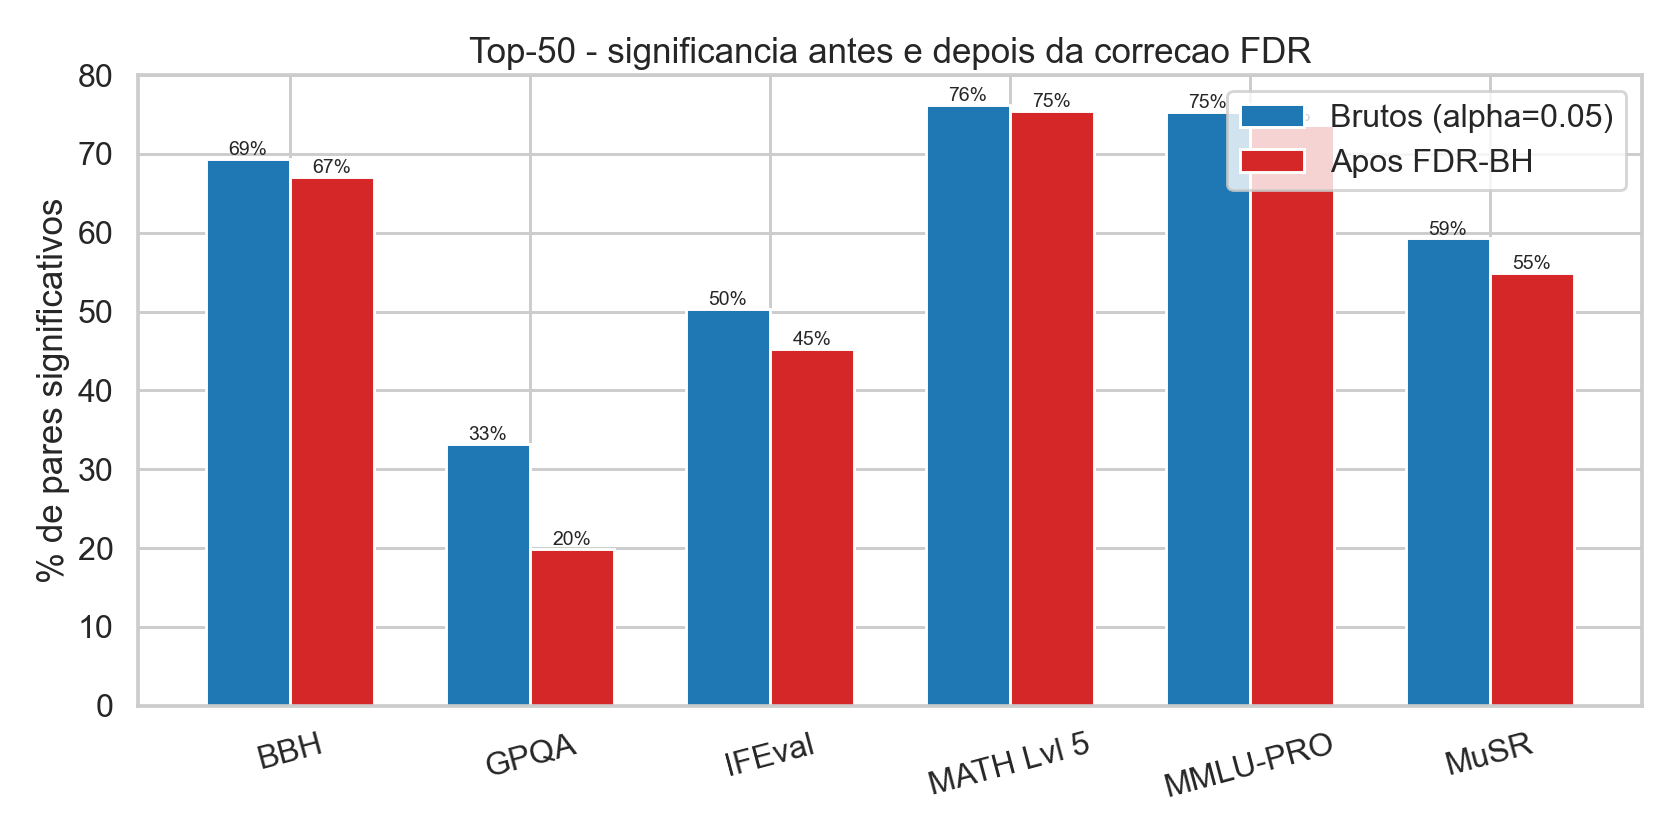
\includegraphics[width=0.8\textwidth]{06_pct_significativos_fdr.png}
\caption{Top-50 pairwise significance before and after Benjamini--Hochberg correction.}
\end{figure}

The effect is most severe in GPQA, where the adjusted fraction of significant top-50 pairs becomes small. This is exactly the pattern expected when many raw discoveries are driven by multiplicity rather than robust separation.

\subsection{Current benchmark sizes are often underpowered for fine ranking}
Using the observed difference between top-1 and top-10 as the target effect, power analysis shows that several benchmarks would need far more items to support precise top-rank distinctions.

\begin{table}[H]
\centering
\caption{Power analysis for separating top-1 from top-10}
\begin{tabular}{lrr}
\toprule
Benchmark & Current \(n\) & Required \(n\) for 80\% power \\
\midrule
GPQA & 448 & \(> 5{,}000\) \\
IFEval & 541 & \(> 3{,}000\) \\
MuSR & 756 & \(> 4{,}000\) \\
MATH Lvl 5 & 1,324 & \(\approx 900\) \\
BBH & 6,511 & \(\approx 500\) \\
MMLU-PRO & 12,032 & \(\approx 300\) \\
\bottomrule
\end{tabular}
\end{table}

This result explains why so many neighboring positions overlap. The issue is not only uncertainty around a single score. It is also lack of power for the specific ranking question people want to answer.

\subsection{Bootstrap favors tiers over exact positions}
Bootstrap resampling of ranking position makes the overlap explicit. Even when models are sorted by median position, their 95\% intervals frequently overlap over many places.

\begin{figure}[H]
\centering
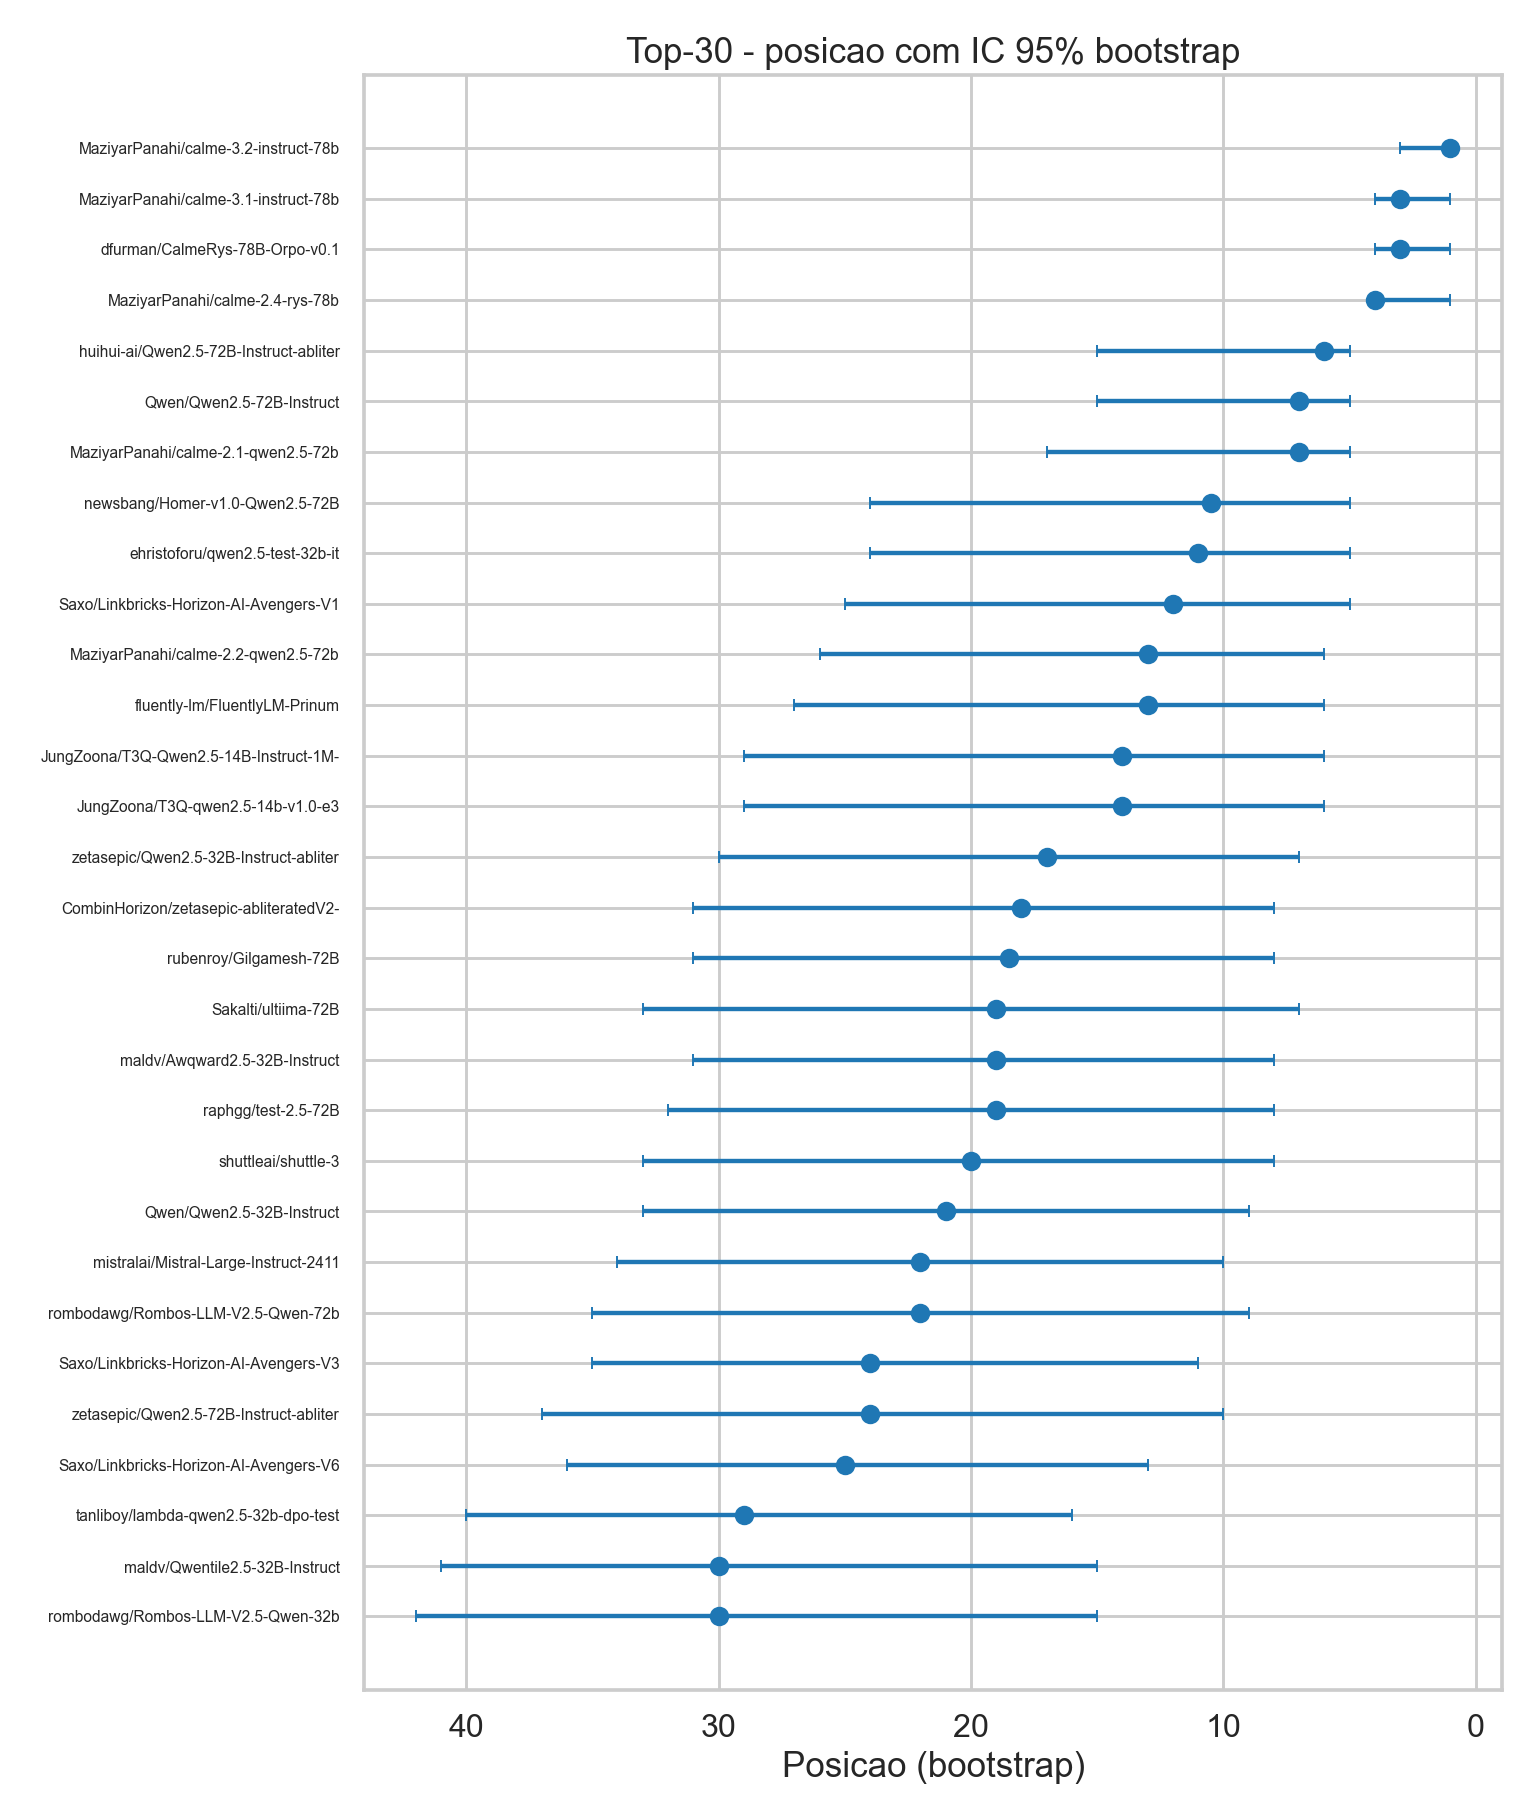
\includegraphics[width=\textwidth]{08_ranking_bootstrap_top30.png}
\caption{Top-30 models with bootstrap median rank and 95\% interval.}
\end{figure}

The ranking is therefore better summarized as a small set of statistical tiers than as dozens of exact, defended positions.

\subsection{Metadata explains most of the visible ordering}
A separate machine-learning experiment regresses leaderboard average on metadata alone. The best-performing model, XGBoost, reaches about \(R^2 = 0.70\) on held-out data. This means that much of the visible ordering is already captured by variables such as parameter scale, architecture family, precision, and organization.

\begin{figure}[H]
\centering
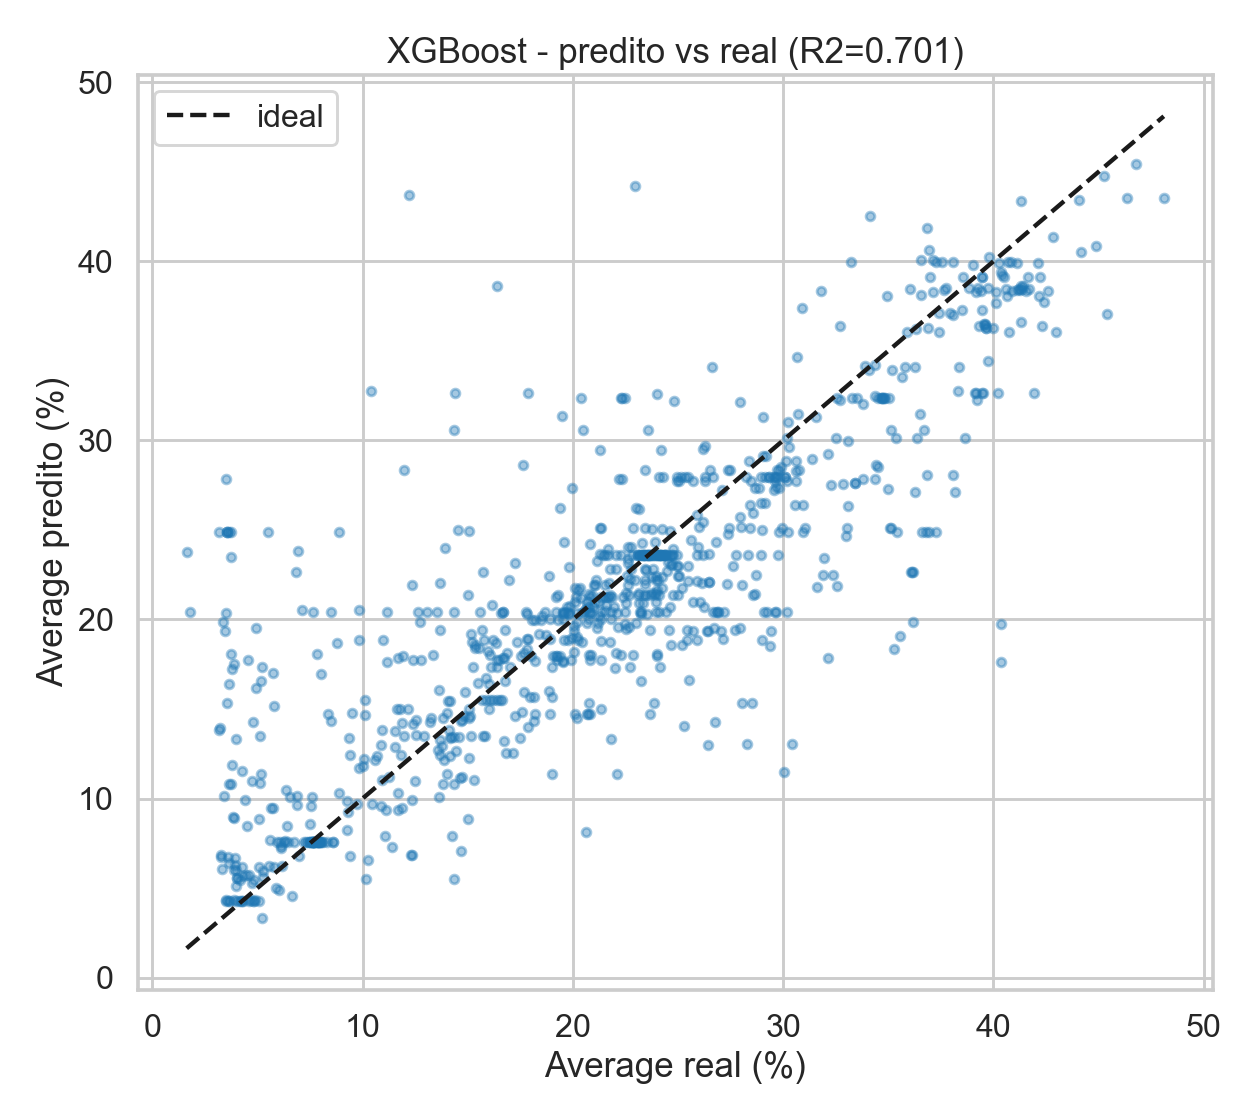
\includegraphics[width=0.78\textwidth]{07_pred_vs_real_xgb.png}
\caption{Leaderboard average predicted from metadata only.}
\end{figure}

This result does not imply that architecture and training details do not matter. It implies that most leaderboard variation at the top is not especially surprising once coarse model metadata is known. The residual is where genuine departures from expectation are likely to live.

\subsection{Arena tells the same broad story}
Arena preference battles were modeled with Bradley--Terry and reported on an Elo-like scale. The top of the Arena separates into a clearer upper tier, but most neighboring models still show overlapping uncertainty intervals.

\begin{figure}[H]
\centering
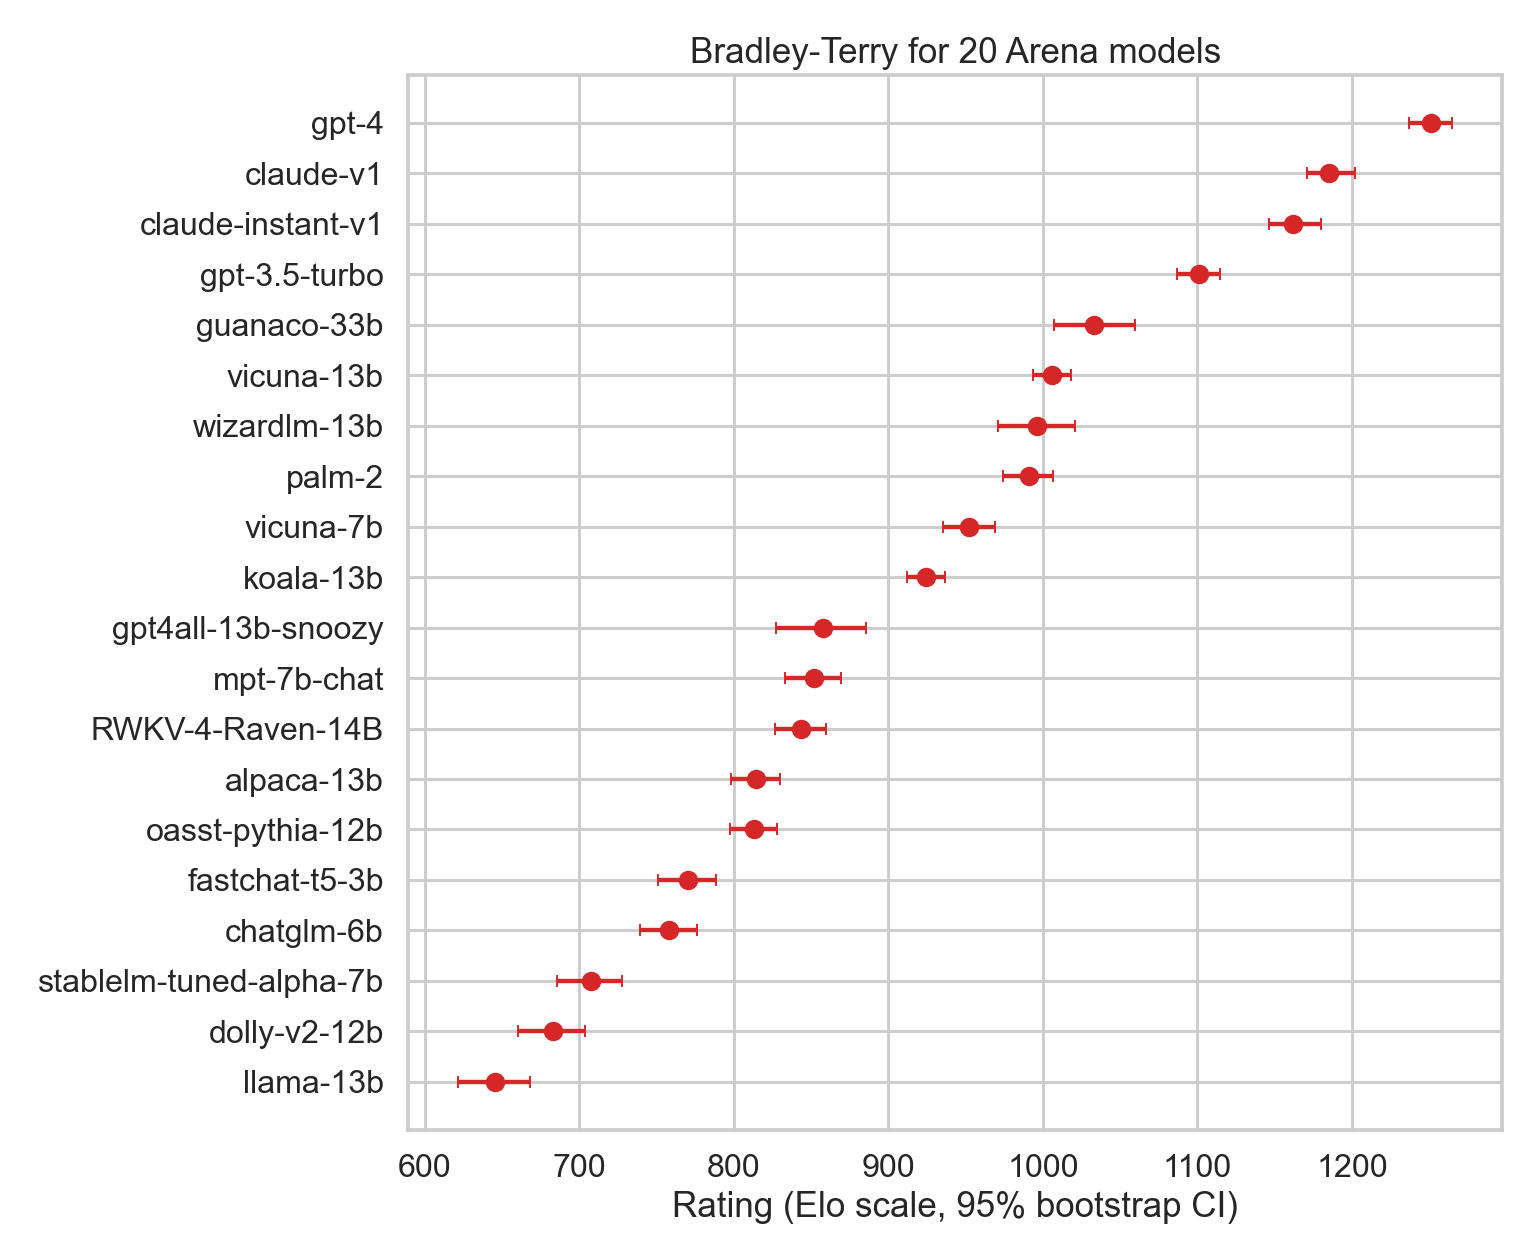
\includegraphics[width=0.82\textwidth]{09_bradley_terry.png}
\caption{Arena Bradley--Terry fit on an Elo-like scale with bootstrap intervals.}
\end{figure}

On the models shared by both datasets, the qualitative ordering is preserved. The overlap is small, but the agreement is informative: large performance gaps appear real across distinct evaluation regimes, while micro-differences remain fragile.

\section{Discussion}
Three conclusions stand out.

First, uncertainty is not a cosmetic addition. It changes the interpretation of the leaderboard itself. In small benchmarks, the confidence interval is often wide enough that consecutive top models cannot be honestly distinguished.

Second, the problem is compounded by multiplicity. Once the number of pairwise tests is acknowledged and FDR control is applied, much of the apparent significance disappears. This means that exact ranking language is often stronger than the data justify.

Third, the most defensible unit of decision is the tier, not the position. The combination of wide score intervals, low power for top-vs-top comparisons, and overlapping bootstrap ranks leads to the same operational recommendation: treat the upper leaderboard as a set of broad, uncertain groups rather than a precise order.

\section{Conclusion}
This project contributes a full statistical re-reading of public LLM rankings. Across benchmark uncertainty, pairwise inference, power analysis, metadata modeling, and Arena comparison, the evidence points in the same direction: exact leaderboard position is often an artifact of reporting precision rather than a stable empirical fact.

For evaluation practice, the implication is modest but important. Public leaderboards remain useful, but they should be read as noisy comparative instruments. When the differences are small, rank should be translated into uncertainty-aware tiers before it is used for product, research, or communication decisions.

\bibliographystyle{plainnat}
\bibliography{../references}

\end{document}
